% This is LLNCS.DOC the documentation file of
% the LaTeX2e class from Springer-Verlag
% for Lecture Notes in Computer Science, version 2.4
\documentclass{llncs}
\usepackage{llncsdoc}
\usepackage{graphicx}
%
\begin{document}

\title{Team description of CIT Brains @Home}

\author{Ryuichi Ueda \and
Yasuo Hayashibara \and
Shinya Fujie \and
Yuya Aoki \and
Hirofumi Inoue \and
Hiroto Matsuzaki \and
Kazuya Natsusako \and
Akie Ohno \and
Yuki Sato \and
Ryo Shimomura \and
Shotaro Terato \and
Kiyoshi Irie
}

\institute{Chiba Institute of Technology,\\
2-17-1 Tsudanuma, Narashino, Chiba, Japan}

\maketitle
%
\begin{abstract}
CIT Brains @Home has been newly set up in November 2016.
We have built a robot for 
\end{abstract}
%
\section{The aim of the team}

CIT Brains @Home has been newly set up in November 2016
by the staff and students in Department of Advanced Robotics,
Chiba Institute of Technology.
The aim of this team is integration of research progresses
in our department.

\begin{itemize}
	\item    Description of the hardware and software including a list of integrated 
	\item    externally available components (including commercial products, freeware, Open Source, etc.) 
	\item    Photo(s) of the robot 
	\item    Focus of research/research interests 
	\item    Applicability of the robot in the real world
\end{itemize}

\section{Robot}
The robot, which has no name, is mainly composed of a commercial mobile robot,
two self-produced manipulators.

\subsection{Hardware}
\subsubsection{Mobile robot part}

We use i-Cart mini\cite{icartmini} as a mobile robot part
with some modifications. In our department, 
this robot is also used for Tsukuba Challenge,
which is an annual competition on outdoor navigation of mobile robots
held in Japan.

Though the motors are very silent, 
they have an ability to make the robot move on public streets.
This mobile robot has two drive wheels whose diameter are 155[mm], 
and one rear caster whose diameter is 100[mm].
Each of the drive wheel is connected to a slient brushless motor.

Under the front bumper, an UTM-30LX-EW Scanning range finder
is attached for navigation.
A Microsoft Kinect at the top of the robot is used for
detecting and following persons.


\subsubsection{Manipulator part}

The robot has two manipulators, which are called arms hereafter.
Each arm has 

\begin{figure}[h]
	\begin{center}
		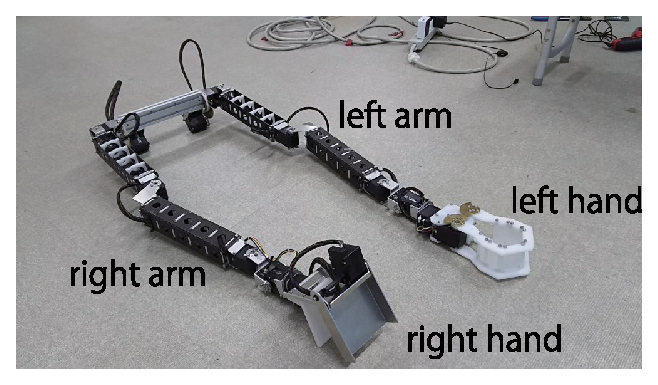
\includegraphics[width=0.7\linewidth]{./IMAGE/manipulators.eps}
		\caption{Manipulators and Hands}
		\label{fig:manipulators}
	\end{center}
\end{figure}


Two kinds of hand are attached to
the manipulators respectively.

\subsubsection{Cover of the robot} We have never been prepared.

\subsection{Software}

\section{Innovative technology and scientific contribution}

Our basic idea to realize home-care robots is that they
should try something even if they have certain information
what they should do. Some mistakes will occur when the robot
acts without certain information.
However, a decision making rule that permits mistakes will make
a robot accomplish more tasks than another rule that waits for
perfect information.

We also think that decision making with this loose policy
will generate a natural communication between a robot and its owners.
For example, a person want to eat cookies
with a high probability when the owner asks his/her robot to bring cookies.
However, there is some some possibility that the owner

\section{Contribution of open source}

We have developed a ROS module for servo motors made by Kondo Kagaku Co., Ltd.


\bibliographystyle{splncs03}
\bibliography{../bibfiles/eng,../bibfiles/url}

\end{document}
